\chapter{Test programs}
\label{test-programs}

There are a number of test programs in the directory
\wfile{test-apps}.  Where possible these are written to be
independent of the target board using configuration files (see
\protect\hyperref[configuration]{configuration}).


\section{USB}
\label{usb-interfacing}

To help debug your programs, it is useful to be able to print values.
This can be achieved by redirecting stdio using the \wikiref{USB
  CDC}{USB CDC} protocol.  For example, here's an example program
\wfile{test-apps/usb_serial_test1/usb_serial_test1.c}.

\inputminted{C}{../../src/test-apps/usb_serial_test1/usb_serial_test1.c}

To get this program to work you need to compile it and program the
SAM4S using:
%
\begin{minted}{bash}
$ cd wacky-racers/src/test-apps/usb_serial_test1
$ make program
\end{minted}

You then need to connect your computer to the USB connector on your PCB.
If you are running Linux, run:
%
\begin{minted}{bash}
$ dmesg
\end{minted}

This should say something like:
%
\begin{verbatim}
Apr 30 11:03:50 thing4 kernel: [52704.481352] usb 2-3.3: New USB device found, idVendor=03eb, idProduct=6202
Apr 30 11:03:50 thing4 kernel: [52704.481357] usb 2-3.3: New USB device strings: Mfr=1, Product=2, SerialNumber=3
Apr 30 11:03:50 thing4 kernel: [52704.482060] cdc_acm 2-3.3:1.0: ttyACM0: USB ACM device
\end{verbatim}

Congrats if you see \texttt{ttyACM0:\ USB\ ACM\ device}!  If not, see
\wikiref{USB_debugging}{USB debugging}.

You can now run a \wikiref{Serial_terminal_applications}{serial
  terminal program}. For example, on Linux:
%
\begin{minted}{bash}
$ gtkterm -p /dev/ttyACM0
\end{minted}

On the Windows machines in the ESL you can use Tera Term. On opening the
application, select the correct \code{COM} port from the \code{Serial}
dropdown. If there are multiple \code{COM} ports listed and you can't
tell which one belongs to the USB serial device, unplug the USB and
observe which \code{COM} port number is added to the dropdown menu when
you reinsert it.

All going well, this will repeatedly print `Hello world'.

If run Linux and get an error `device is busy', it is likely that the
ModemManager program has automatically connected to your device on the
sly. This program should be disabled on the ECE computers. For more
about this and using other operating systems, see \wikiref{USB
CDC}{USB CDC}.

The test apps:
\begin{itemize}
   \item \wfile{test-apps/usb_serial_test1}
   \item and \wfile{test-apps/usb_serial_read}
 \end{itemize}
both contain examples of \emph{reading} commands from the USB
interface. This can be useful for debugging: for example you can
control the motor speed by sending commands to your board via the
serial interface. To get serial input playing nicely on your
development machine, you need to enable local echo and use newlines as
line endings in your serial terminal program. This is configured on
the aforementioned terminal programs as follows.
\begin{description}
  \item[Tera Term] Open the \verb|Setup > Terminal...|
  menu, check \verb|Local echo|, and set the \verb|New-line| setting
  to \verb|LF| for transmit and receive. See \reffig{tera-term-setup}.

  \item[gtkterm] In the \verb|Configuration| dropdown menu, make sure
  \verb|Local echo| and \verb|CR LF auto| are checked.
\end{description}

\begin{figure}[h]
  \centering
  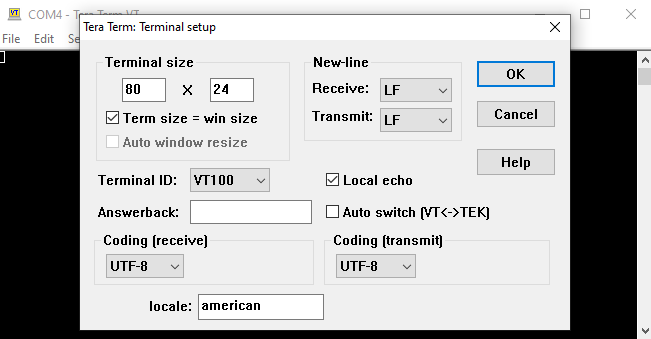
\includegraphics{figs/tera-term-setup.png}
  \caption{Tera Term setup for local echo with newlines (aka line
  feeds [LF]).}
  \label{fig:tera-term-setup}
\end{figure}

\section{PWM}
\label{pwm-test}

The program \wfile{test-apps/pwm_test2/pwm_test2.c} provides an
example of driving PWM signals.

\inputminted{C}{../../src/test-apps/pwm_test2/pwm_test2.c}

Notes:
%
\begin{enumerate}
\item
  This program is for a different H-bridge module that requires two
  PWM signals and forward/reverse signals. You will need to generate
  four PWM signals or be clever with two PWM signals.

\item
  The \code{pwm_cfg_t} structure configures the frequency, duty cycle
  and alignment of the output PWM.

\item The frequency is likely to be too high for your motor.

\item \code{pwm_channels_start} is used to start the PWM channels
  simultaneously.
\end{enumerate}

If the program does not work, see  \hyperref[debugging-pwm]{PWM debugging}.

To drive the motors you will need to use a bench power supply. Start
with the current limit set at 100\,mA maximum in case there are any
board shorts.  When all is well, you can increase the current limit;
you will need at least 1\,A.

\section{Accelerometer}
\label{accelerometer-test}

The ADXL345 accelerometer connects to the SAM4S using the I2C bus (aka
TWI bus).  The program
\wfile{test-apps/accelerometer_test1/accelerometer_test1.c} provides
an example of using the ADXL345 accelerometer.  All going well, this
prints three 16-bit acceleration values per line to USB CDC. Tip your
board over, and the the third (z-axis) value should go negative since
this measures the effect of gravity on a little mass inside the
accelerometer pulling on a spring.

If the program does not work, the main reasons are:

\begin{enumerate}
\item
  You have specified the incorrect address.  Set
  \code{ADXL345_ADDRESS} to either \code{0x1D} or \code{0x53} in
  \file{target.h} depending on the state of the \verb|ALT ADDRESS| pin
  on the chip (see datasheet).
\item
  You are using TWI1. The \pin{PB4} and \pin{PB5} pins used by TWI1
  default to JTAG pins. See
  \protect\hyperref[disabling-jtag-pins]{disabling JTAG pins}.
\end{enumerate}
%
See also \protect\hyperref[checking-accelerometer]{accelerometer checking}.


\section{Radio}
\label{radio-test}

The program \wfile{test-apps/radio_tx_test1/radio_tx_test1.c} provides
an example of using the radio as a transmitter.

The companion program
\wfile{test-apps/radio_rx_test1/radio_rx_test1.c} provides an example
of using the radio as a receiver.

\inputminted{C}{../../src/test-apps/radio_rx_test1/radio_rx_test1.c}


Notes:
%
\begin{enumerate}
\item Both programs must use the same RF channel and the same address.

\item Some RF channels are better than others since some overlap with
  WiFi and Bluetooth.

\item The address is used to distinguish devices operating on the same
  channel. Note, the transmitter expects an acknowledge from a
  receiver on the same address and channel.

\item The number of bytes that can be transmitted is set by the
  \code{payload\size} field in the configuration structure.  This has a
  maximum value of 32.

\item The radio `write` method blocks waiting for an
  auto-acknowledgement from the receiver device. This acknowledgement
  is performed in hardware. If no acknowledgement is received, it
  retries for up to 15 times. The auto-acknowledgement and number of
  retries can be configured in software.

\item If the program hangs in the \code{panic} loop, there is no
  response from the radio module, check SPI connections and see
  \hyperref[debugging-spi]{SPI debugging}.

\item The radio has two modes: transmit and receive.  Calling
  \code{nrf24_write} switches to transmit mode and calling
  \code{nrf24_read} switches to receive mode.

\end{enumerate}

If you cannot communicate between your hat and racer boards, try
communicating with the radio test modules Scott Lloyd has in the SMT
lab.


\section{ADC}
\label{ADC}

\wfile{test-apps/adc_usb_serial_test2/adc_usb_serial_test2.c} shows
how to read from two multiplexed ADC channels, specifically the hat joystick
channels (although it can be adapted for different purposes).  For more details
see \wfile{mat91lib/adc/adc.h}.

\inputminted{C}{../../src/test-apps/adc_usb_serial_test2/adc_usb_serial_test2.c}

If the program does not work, see  \hyperref[debugging-adc]{ADC debugging}.

The ADC can be also set up to stream data continuously but you need to
use interrrupts or DMA.


\section{Pushbutton}
\label{pushbutton}

\wfile{test-apps/button_test1/button_test1.c} shows the use of a
simple button driver to read a pushbutton.  This driver does not debounce the button.

\inputminted{C}{../../src/test-apps/button_test1/button_test1.c}

\wfile{test-apps/button_test2/button_test2.c} shows the use of a
simple button driver to read a pushbutton.  This driver does button
debouncing and state-transition detection.  For more details see
\wfile{mmculib/button/button.h}.

\inputminted{C}{../../src/test-apps/button_test2/button_test2.c}


\section{LEDtape}
\label{ledtape}

\wfile{test-apps/ledtape_test1/ledtape_test1.c} shows how to drive the
LEDtape.  Note, the timing is not consistent for all LED tapes so you
may need to change \code{LEDTAPE_PERIOD} in \file{target.h}.

\inputminted{C}{../../src/test-apps/ledtape_test1/ledtape_test1.c}


\wfile{test-apps/ledtape_test2/ledtape_test2.c} uses a more
sophisticated means of controlling the LEDs.

\inputminted{C}{../../src/test-apps/ledtape_test2/ledtape_test2.c}
